%%%%%%%%%%%%%%%%%%%%%%%%%%%%%%%%%%%%%%%%%%%%%%%%%%%%%%%%%%%%%%%%%
%  _____   ____  _____                                          %
% |_   _| /  __||  __ \    Institute of Computitional Physics   %
%   | |  |  /   | |__) |   Zuercher Hochschule Winterthur       %
%   | |  | (    |  ___/    (University of Applied Sciences)     %
%  _| |_ |  \__ | |        8401 Winterthur, Switzerland         %
% |_____| \____||_|                                             %
%%%%%%%%%%%%%%%%%%%%%%%%%%%%%%%%%%%%%%%%%%%%%%%%%%%%%%%%%%%%%%%%%
%
% Project     : LaTeX doc Vorlage für Windows ProTeXt mit TexMakerX
% Title       : 
% File        : vorgehen.tex Rev. 00
% Date        : 7.5.12
% Author      : Remo Ritzmann
% Feedback bitte an Email: remo.ritzmann@pfunzle.ch
%
%%%%%%%%%%%%%%%%%%%%%%%%%%%%%%%%%%%%%%%%%%%%%%%%%%%%%%%%%%%%%%%%%

\chapter{Approach and Methodology}\label{chap.vorgehen}
\section{Basic Considerations}\label{basic_cons}
As described under \autoref{baseline}, our work is based on the work of S. Huschauer \cite{flatland}. We take the idea of using the A3C algorithm to solve the flatland problem and try various modifications in an attempt to improve its performance.\\
We proceed by giving an intution, what we want to achieve by changing the specified part, followed by an experiment to either prove or disprove our hypothesis.\\
For training purposes, we started by reimplementing the algorithm by ourselfes. This enabled us from the beginning to gain a deeper understanding of how the algorithm works and where we could find possible areas for improvement. From there, we iteratively added these potential improvements to later compare them against the version without this feature.

\subsection*{Reproducability in Reinforcement Learning}\label{enhanced_observations}
It is important to note, that the training process of reinforcement learning and especially multi agent reinforcement learning is hard to evaluate and reproduce. Depending on the initial weights of the neural networks and the shape of the environments, the performance may vary on each restart. Also, the number of workers can 
significantly influence the training performance. To counter the latter, we execute all presented experiments on machines with the same specifications (see TODO-INFRASTRUCTURE).



\section{Reinforcement Learning for Flatland}
\subsection*{A3C Implementation}\label{enhanced_observations}
Originally, the asynchronous advantage actor critic algorithm (A3C) has been designed for use in a single agent environment \cite{a3c}.
By applying it in a multi agent environment, we implicitly convert the environment into a non-stationary environment.
While applying A3C in a multi agent setting, the other agents can be viewed as part of the environment. This means, the behaviour of the environment changes while training, due to the fact that the behaviour of the other agents changes.

Gupta et al. \cite{multiagent_comp_a3c_dqn_etc} finds, that RL methods like Deep-Q networks (DQN) and Trust region policy optimization (TRPO) are not performing well in a multi agent environment, due to the combination of experience replay and non-stationarity of the environment. We therefore suggest, that it is not recommendable to keep an experience replay buffer with older episodes. Otherwise the sampled experience might represent old agent behaviour which is then learned.

\subsection*{Observation Design}\label{enhanced_observations}
The flatland environment provides a base to build custom observation builders that can be used to create a state representation for the agents. Based on the provided TreeObsForRailEnv (see \autoref{observations}), we implement a custom observation builder which we use to produce an input vector to our neural network. This observation builder takes the the current state of the environment and produces a fixed size numeric vectors with values between 0 and 1 for each agent. This input vector should fulfil an number of requirements:
\begin{itemize}
	\item Each rail section the agent possibly rides on next should be visible to the agent.
	\item The agent should be able to detect, whether there is another train coming the opposite direction on any section.
	\item The agent should be able to detect on each switch which turn is closer to his target.
	\item On switches, the agent should be able to see if a turn does lead to his target, even if it is not the fastest way. If this is the case, taking this turn might even be a good option to evade possibly blocking situations.
	\item For the next grid tile, the agent should be able to detect if it is a switch and if so, if it is one the agent can make a decision on. (see \autoref{flatland_intro} for non-usable switches).
	\item 
\end{itemize}

\subsection*{Action Space Reduction and Script Policy Actions}\label{reduced_action_space}
The flatland environment is designed in a way to resemble a classical RL environement. This means, on every timestep, we receive observations for each agent, calculate an action and hand this action to the environment, visible in pseudocode \autoref{alg:no_reduction}. 

\begin{algorithm}[H]
\KwData{initialized flatland environment $\mathcal{E}$, initial observation $\mathcal{s\SPSB{a}{t=0}}$ for all agents }
\KwResult{flatland environment at timestep $\mathcal{t +1}$}
\While{episode not terminal}{
	create empty action array $\mathcal{A}$\\
	\For{every agent $\mathcal{a}$}{
		get current state $\mathcal{s\SPSB{a}{t}}$ of agent\\
		Fetch action  $\mathcal{u}$ for agent $\mathcal{a}$ at timestep $\mathcal{t}$ based on $\mathcal{s\SPSB{a}{t}}$ from policy $\pi$\\
		$\mathcal{A[a]}$ = $\mathcal{u}$
	}
	call $\mathcal{step(A)}$ of $\mathcal{E}$\\
	retrieve reward $\mathcal{R}$\\
	retrieve all new states $\mathcal{s_{t+1}}$\\
}
\caption{Default episode for flatland environment}
\label{alg:no_reduction}
\end{algorithm}
While this makes sense in an environement where agents need to take an action on every timestep (such as Atari games), in flatland most of the time the only reasonable action is to move forward as visible in \autoref{fig:no_desicion}. Only around switches, the actions of an agent have acutual consequences.
\begin{figure}
	\centering
	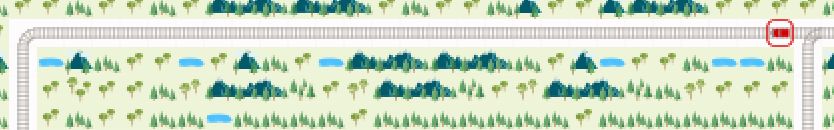
\includegraphics[width=300pt]{images/screenshot_no_decision.png}
	\caption{Screenshot from flatland environment. A train heading east. The only reasonable action is to ride forward.}
	\label{fig:no_desicion}
\end{figure}
Every action that is produced by the neural network should be included for training, so the network can adapt to this type of situation. The problem arises now, that all these actions of riding forward are included into the training of the agent. The influence of the actions that actually matter (e.g. the ones around switches) is thereby not as big as it could be, because a large portion of the training data is actually situations that do not actually require decisions.\\
To solve this problem, we implement hard coded rules that the agents follow as long as they are not in a situation to make a decision. We  Only around switches, the neural network policy is activated. As a consequence, the data used for training has less samples but the samples available are of higher quality. The training with this mechanism implemented looks like TODO: Ref to algorithm.

\begin{algorithm}[H]
	\KwData{initialized flatland environment $\mathcal{E}$, initial observation $\mathcal{s\SPSB{a}{t=0}}$ for all agents }
	\KwResult{flatland environment at timestep $\mathcal{t +1}$}
	\While{episode not terminal}{
		create empty action array $\mathcal{A}$\\
		\For{every agent $\mathcal{a}$}{
			get current state $\mathcal{s\SPSB{a}{t}}$ of agent\\
			Fetch action  $\mathcal{u}$ for agent $\mathcal{a}$ at timestep $\mathcal{t}$ based on $\mathcal{s\SPSB{a}{t}}$\\
			$\mathcal{A[a]}$ = $\mathcal{u}$
		}
		call $\mathcal{step(A)}$ of $\mathcal{E}$\\
		retrieve reward $\mathcal{R}$\\
		retrieve all new states $\mathcal{s_{t+1}}$\\
	}
	\caption{Default episode for flatland environment}
	\label{alg:no_reduction}
\end{algorithm}

 This drastically improves training performance.

// TODO: Chart


\subsection*{Curriculum Learning and Reward assignment}\label{curriculum_learning}
The reward assignment in flatland can be freely configured. But as long as there is not some distance-to-target dependent reward function, the probability, that an agent with an uninformed policy finds its target is small. This is especially the case for large environments with many trains on it. For example, most evaluation environments of flatland round 2 have up to 200 individual agents and are up 100x100 tiles large (SOURCE!). The rollout of such an environment takes a lot more time than the rollout of a 20x20 environment with 5 trains. Also, the probability, that a train arrives in a small environement is larger and therefore, the experience is more valuable for training.
To improve training times, it makes therefore sense to start with a small environment and move to larget ones, once the agents mastered pathfinding and basic collision avoidance.

\subsection*{Entropy Balancing and Hyperparameter Tuning}\label{enhanced_observations}
In RL, it is of great importance to find the right combination of exploration and explotation. During exploration, the agent explores as much of the state space as possible. This enables the agent to later exploit the found states which are beneficial. Without this exploration, there is a chance that the agent settles on suboptimal policies too quickly and ignores parts of the state space the agent has never seen.\\
The policy is characterized by a probability distribution of actions.


\subsection*{Agent Communication}\label{reduced_action_space}
Communication in multi agent RL is a topic of active research and considered very complex


\section{Distrubuted Architecture and Parallelism}\label{dist_architecture}
Für die vorliegende Arbeit wurden die unten aufgeführten Programme eingesetzt.








\begin{itemize}
\item (Beschreibt die Grundüberlegungen der realisierten Lösung (Konstruktion/Entwurf) und die Realisierung als Simulation, als Prototyp oder als Software-Komponente)
\item (Definiert Messgrössen, beschreibt Mess- oder Versuchsaufbau, beschreibt und dokumentiert Durchführung der Messungen/Versuche)
\item (Experimente)
\item (Lösungsweg)
\item (Modell)
\item (Tests und Validierung)
\item (Theoretische Herleitung der Lösung)
\end{itemize}

\section{(Used Software)}\label{software}
We used the following tools in our project.

\subsection*{Working Environment}\label{os}
\begin{itemize}
	\item Microsoft Windows 10
	\item Ubuntu 19.04
\end{itemize}

\subsection*{Visual Studio Code}\label{vsc}
\begin{itemize}
	\item Visual Studio Code 1.40
\end{itemize}

\subsection*{Documentation}\label{dokutools}
\begin{itemize}
	\item XeLateX with Visual Studio Code
	\item XeLateX with WebStorm
\end{itemize}


\subsection*{Programming language}\label{programminglanguages}
\begin{itemize}
	\item Python 3.6
\end{itemize}

\subsection*{Python modules}\label{modules}
\begin{itemize}
	\item Flatland-rl 1.3 - 2.1.10
	\item Tensorboard 2.0
	\item Keras x.x
	\item Cython x.x
	\item %TODO: finish this
\end{itemize}


\section{Basic considerations}
%split into round 1 / round 2

\subsection{Round 1}
%Observations
%Convolutional network + Global observations
%Early stopping
%Reward vergabe angepasst
We started with rebuilding the A3C algorithm from S. Huschauer to get a better knowledge how A3C works.\\
We made some experiments with different observations: TreeObservations and GlobalOberservations.
Because we made better and faster progress with GlobalObservatione we continued with those and combind them with a convolutional network.
Right after starting this project, we faced a problem regarding the reward distribution.\\


\subsection{Round 2}




\section{Measurands}
%Messgrössen: Evaluator, benchmark

\section{Experiments}
%

\section{Solution approach}
%Neue Actions


\section{Testing and submissions}

\section{Theoretical derivation of the solution}



